%\documentclass[a4paper,11pt]{article}
\documentclass[a4paper,11pt]{scrartcl}

\usepackage[utf8]{inputenc}
\usepackage[italian]{babel}

\usepackage{graphicx} %for includng images
\graphicspath{{img/}}

\usepackage{siunitx} % package for deciBel and other units

\usepackage{amsmath} % package for ``cases'' and other matemagical stuff

\usepackage{circuitikz} % circuit drawer

\usepackage{subcaption}  %per immagini multiple

%\usepackage{xcolor} % Colori!
\usepackage{colortbl} %colori nelle tabelle!!

\usepackage{multirow} %righe doppie nelle tabelle

\usepackage{makecell} %multirow box

\title{Appunti di compatibilità elettromagnetica}
\author{Daniele Olivieri}
\date{}

\pdfinfo{%
  /Title    ()
  /Author   ()
  /Creator  ()
  /Producer ()
  /Subject  ()
  /Keywords ()
}
\includeonly{lezione12_09_04,lezione13_11_04}
\begin{document}
\maketitle
\setlength\arrayrulewidth{1.2pt} %larghezza righe tabelle
\section{Cenni sulla compatibilità elettromagnetica}
\paragraph{Definizione}
La compatibilità elettromagnetica è la scienza che studia la capacità di qualsiasi 
apparecchiatura di funzionare in modo soddisfacente in un ambiente soggetto a disturbi elettromagnetici
senza produrre disturbi intollerabili ad altri apparati.

Ad esempio quando si avvicina il cellulare alle casse dello stereo, si percepisce un ronzio nella cassa
dello stesso, questo fenomeno è dovuto al trasferimento di parte dell'energia emessa dal cellulare ai cavi 
dello stereo che lo convertono in disturbo sonoro.
Questo fenomeno non può e non deve avvenire nemmeno in situazioni critiche come una sala ospedaliera in cui il disturbo
emesso da un cellulare potrebbe alterare le misurazioni effettuate da un apparecchio come l'elettrocardiografo.
Il dispositivo elettromedicale deve essere reso immune dai disturbi. (Immagina un pacemaker!)

Si distingue la Compatibilità in senso attivo o passivo:
\begin{itemize}
 \item Attivo: l'oggetto non deve emettere disturbi di entità troppo elevata
 \item Passivo: l'oggetto deve essere in grado di resistere ai disturbi esterni, emessi da altri dispositivi
 senza alterare il proprio funzionamento
\end{itemize}

Altri dispositivi che devono sottoporsi alle analisi di Compatibilità sono i dispositivi comunque complessi
composti ad esempio da parti multiple, che possono essere commercializzate separatamente. In questo caso solo
le singole parti devono garantire un soddisfacimento dei vincoli dati dalla Compatibilità Elettromagnetica.

Si parla di Compatibilità \textbf{intra-sistema} se si analizza il problema all'interno del sistema con approccio
``microscopico'', la compatibilità \textbf{inter-sistema} analizza invece la compatibilità tra dispositivi differenti.
Esistono due grandi fenomeni: \textbf{emissione} e \textbf{immunità}, questi due fenomeni richiamano la compatibilità in senso attivo e passivo.
\medskip

I disturbi vengono poi caratterizzati in disturbi \textbf{radiati} in aria e disturbi \textbf{condotti} tramite
un canale vincolato, ad esempio un cavo di alimentazione.
Nessun disturbo si può caratterizzare mediante una singola tipologia, %rivedi qui
un disturbo radiato ad esempio può accoppiarsi con il cavo di alimentazione e diventare disturbo condotto.
Il cilindro di ferrite presente su un cavo VGA ad esempio attenua i disturbi che tendono a propagarsi lungo il cavo
incrementandone l'impedenza.
\newpage
Al di sotto dei 30 MHz si ritiene che il fenomeno sia di natura prevalentemente condotta,
al di sopra invece si ritiene il fenomeno di natura radiata. Ad esempio il ``\textbf{surge}'' nasce da un fulmine e si
propaga per via radiata, ma raggiunge i dispositivi mediante i loro cavi di alimentazione.

I problemi di compatibilità intra-sistema vengono gestiti durante la fase di progettazione del dispositivo
ad esempio mediante una corretta disposizione delle piste del circuito, attraverso una opportuna scelta dei 
componenti oppure mediante una schermatura interna, non disporrò mai un dispositivo molto suscettibile
in prossimità di un potenziale emettitore di disturbi sulla stessa scheda elettronica.

La compatibilità inter-sistema viene studiata mediante una caratterizzazione dell'ambiente elettromagnetico, 
mediante una classificazione delle sorgenti dei disturbi e delle vittime, attraverso la definizione dei livelli di massima
emissione e minima immunità, non riguarda soltanto l'oggetto ma anche la sua posizione nell'ambiente
elettromagnetico.
\medskip

L'\textbf{ambiente elettromagnetico} è l'insieme di tutti i fenomeni elettromagnetici osservabili in un
determinato luogo, sostanzialmente il \textbf{campo} elettromagnetico, le condizioni al contorno e le caratteristiche
del mezzo in cui i disturbi si propagano. Per modellare l'ambiente e ottenere un risultato valido
è necessaria una esatta conoscenza di tutti questi parametri, impresa per nulla semplice.

Anzichè calcolare la soluzione numericamente, si preferisce infatti misurare direttamente l'ambiente
elettromagnetico e le emissioni generate dall'oggetto. Anche quest'aspetto presenta dei problemi come
l'incertezza di misura e la discretizzazione del fenomeno, ovvero la scelta del numero di punti in cui effettuare
la misura.
Si può scegliere di eseguire entrambe le procedure, utilizzare un modello numerico approssimato per 
prevedere a grandi linee i risultati e approfondire con le misurazioni i punti più critici.

\paragraph{La perturbazione elettromagnetica}
È un fenomeno di origine elettromagnetico capace di alterare il funzionamento di un'apparecchiatura,
può essere costituito da:
\begin{itemize}
\item Rumore
\item Segnale non desiderato
\item Alterazione del mezzo
\end{itemize}


\section{Un pò di storia}
%\paragraph{}
A partire dal 1920 si diffondono i primi articoli riguardanti le interferenze radio, dando il via alla ricerca
sui problemi di compatibilità elettromagnetica.
Dieci anni dopo, con lo sviluppo delle industrie che utilizzavano energia elettrica si sono evidenziati i fenomeni
di disturbo e interferenza dovuti alle linee elettriche ferroviarie e all'utilizzo dei motori elettrici.
Durante la II Guerra Mondiale l'utilizzo di comunicazioni radio e sistemi radar fu cruciale per la riuscita
delle missioni, iniziò una vera e propria guerra tecnologica e ci si rese conto della necessità di regolamentare
le trasmissioni sulle varie frequenze.

Tra gli anni '50 e '70 si diffusero i transistor e l'elaborazione digitale dei dati, i circuiti divenivano
sempre più piccoli e commutavano a frequenze sempre più elevate. Questi segnali ad alte frequenze generavano numerosi
disturbi a banda larga in spazi molto ravvicinati fra i vari componenti.

\paragraph{Timeline essenziale} della compatibilità elettromagnetica:

\begin{itemize}
 \item \textbf{1923}: Primi rapporti tecnici sulle interferenze radio
 \item \textbf{1933}: Prime riunioni internazionali per la regolamentazione delle radio interferenze, IEC-UIR
 \item \textbf{1934}: Costituzione del CISPR, con prima riunione a Giugno
 \item \textbf{1979}: Documento da parte della FCC per la limitazione delle emissioni EM dei dispositivi digitali
\end{itemize}


In \textbf{Europa}: 
\begin{itemize}
 \item \textbf{1989}: Direttiva 89/336 in cui si obbligavano i produttori ad occuparsi della 
 Compatibilità Elettromagnetica, modificata da direttive successive nel 92, 93 ed entrò definitivamente in vigore
 nel Gennaio del 1996.
 \item \textbf{1996}: Recepimento in \textbf{Italia} con Decreto Legislativo n° 615.
 \item \textbf{1997-1998}: Pubblicazione delle \textit{guide di applicazione} UE e CEI per interpretare la Direttiva
 Europea.
 \item \textbf{CT 210}: Viene costituito il comitato tecnico 210 nel CENELEC e nel CEI riguardo la compatibilità
 elettromagnetica.
 \item \textbf{108/04/CE}: Direttiva a valle del progetto \textit{SLIM} al fine di semplificare la legislazione.
\end{itemize}

\paragraph{La direttiva Europea}
Documento mediante il quale l'Unione regola il commercio nel Mercato Interno, il produttore di un'apparecchiatura
deve fornire una \textit{``Dichiarazione di Conformità''} contenuta nel \textit{``Technical Construction
File''} che descriva il prodotto e ne illustri la conformità al fine di ottenere il marchio \textbf{CE}.

Nel \textit{1997} l'iniziativa nota come \textbf{SLIM} (Simplified Legislation for the Internal Market)
evidenziò la necessità di semplificare le normative mantenendo comunque un elevato livello di sicurezza.

Nel ``Nuovo Approccio'' la direttiva indica solo quali sono gli obiettivi da raggiungere ma non come farlo
per non limitare il progresso tecnologico. Le specifiche tecniche da rispettare vengono poi illustrate
nelle Norme Armonizzate, emanate da organizzazioni come il CENELEC, risulta in questo modo molto più semplice
aggiornare una Norma Armonizzata per modificare, ad esempio, i range di frequenza piuttosto che agire sull'intera 
Direttiva Europea, che richiederebbe un lavoro politico e burocratico molto più intenso.

\section{Gli apparati coinvolti}
L'articolo 2.1 della direttiva 108/04/CE distingue:
\begin{itemize}
 \item \textbf{Apparecchiatura}: Ogni apparecchio o impianto fisso
 \item \textbf{Apparecchio}: Dispositivo finito o combinazione di dispositivi finiti, commercializzati come unità 
 funzionali e destinati all'utente finale
 \item \textbf{Impianto fisso}: Combinazione particolare di apparecchi assemblati ed installati per essere
 utilizzati in un solo luogo
\end{itemize}

I dispositivi interessati coprono una grande varietà di settori, a partire dagli elettrodomestici agli apparecchi
per l'informazione, gli apparati per l'illuminazione, le macchine industriali fino alle apparecchiature 
elettromedicali.

La verifica della conformità \textbf{EMC} viene eseguita seguendo le Norme Armonizzate e il risultato delle prove viene
riportato nel \textit{Technical Construction File}, i prodotti che rispettano gli standard di prodotto, (o in assenza
di questi gli standard generici) vengono ritenuti conformi alla direttiva EMC e per questo viene prodotta la
dichiarazione di conformità e rilasciato il marchio CE.
Non è richiesta la marchiatura CE per le installazioni fisse dato che non devono essere commercializzate
tra i paesi membri ma devono solo garantire il corretto funzionamento nel punto in cui vengono installate.
La dichiarazione di conformità può prevedere una autocertificazione o l'intervento di un'autorità esterna per la
revisione della documentazione.

La differenza fra l'autocertificazione o l'intervento dell'autorità esterna è determinata dalla criticità del settore
in cui l'apparecchiatura deve funzionare (es. ambienti medicali, militari ecc...).

La verifica della conformità alla Direttiva EMC non solo consente il libero scambio di prodotti nel mercato europeo
ma permette comunque di realizzare un prodotto di livello superiore, con una maggiore robustezza ai disturbi e una
maggiore compatibilità anche in ambienti elettricamente ``affollati''.

\section{Gli organismi coinvolti}
Nel controllo del rispetto della Direttiva Europea sono coinvolti numerosi organismi e autorità:
Le \textbf{Autorità Competenti} sono enti riconosciuti dai singoli stati ai quali è stato affidato il compito
di vigilare sul mercato e controllare i prodotti che vi transitano, ad esempio le \underline{Camere di commercio}

Gli \textbf{Organismi Competenti} dimostrano di avere le competenze tecniche per verificare le caratteristiche di un 
apparato. Non eseguono le misurazioni sugli apparecchi ma sono in grado di analizzare e valutare
i risultati delle stesse.

Gli \textbf{Organismi Notificati} a cui è demandata, da parte delle Autorità Competenti, la verifica delle
caratteristiche di conformità alla direttiva EMC mediante le misure. Le certificazioni rilasciate dagli organismi
notificati sono già ritenute valide dalla Comunità Europea.

Un organismo competente o notificato deve avere disponibilità di attrezzatura specifica e personale specializzato,
non deve avere alcun conflitto di interessi con l'azienda che richiede la certificazione; deve essere sottoposto a 
verifica periodica. Le sue dichiarazioni hanno validità legale e deve essere assicurato sulla responsabilità civile
delle proprie dichiarazioni.

\begin{figure}[h]
 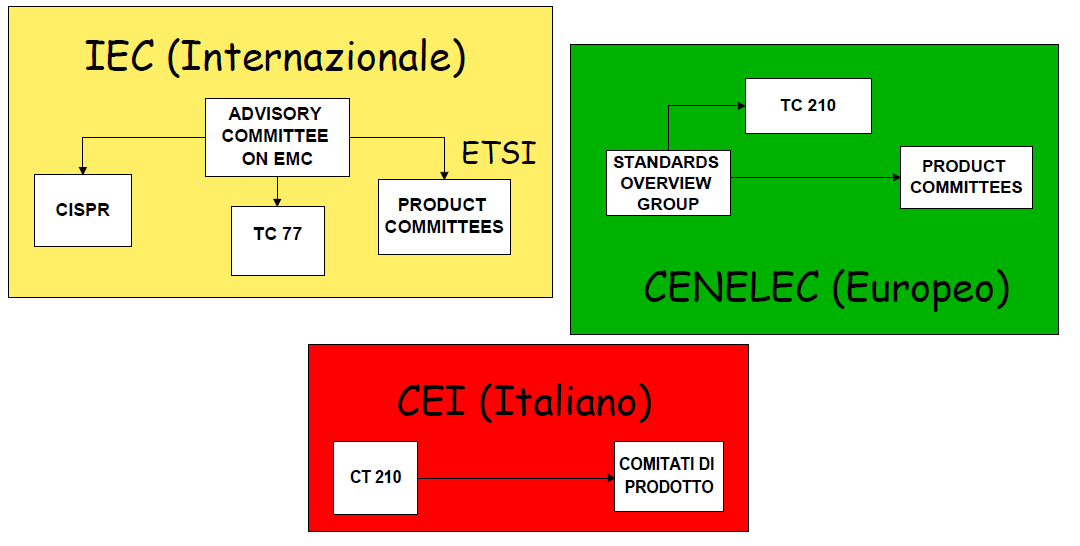
\includegraphics[width=0.7\linewidth]{enti.png}
 \centering
 \caption{Organismi di Normazione}
 \label{fig:enti}
\end{figure}

Tutti i paesi interessati partecipano all'IEC, le Norme attuate in Europa vengono invece rilasciate dal CENELEC mentre
il CEI in Italia collabora con i comitati di prodotto per redigere le norme.
L`IEC non è gerarchicamente superiore al CENELEC, nonostante sia un comitato internazionale non ha potere
sull'Europa, deve essere il CENELEC a recepire ed armonizzare una eventuale norma rilasciata dall'IEC.
L'Italia può avere una propria normazione tecnica ma se ci dovessero essere norme in contrasto con le normative 
Europee, queste dovranno essere aggiornate ed adeguate alla normazione più generale (europea). In teoria il singolo
Stato potrebbe avere normative più stringenti, ma queste potrebbero portare a ricorsi da parte dei produttori
che non potrebbero vendere i loro prodotti nei determinati stati membri, nonostante siano ``a norma''
secondo la Comunità Europea.

\paragraph{Il CISPR} È la commissione internazionale sui radiodisturbi, composta da vari sottocomitati: A,B,D,F,H,I.
%aggiungi elenco
\begin{itemize}
 \item \textbf{CISPR A}: Misure di interferenze radio e metodi statistici di misura.
 \item \textbf{CISPR B}: Interferenze dovute ad apparecchi industriali, scientifici, medicali, apparecchi ad alta tensione e
 apparecchi destinati alla mobilità elettrica.
 \item \textbf{CISPR D}: Disturbi dovuti a strumentazione elettrica/elettronica presente sui veicoli e tutti i dispositivi
 alimentati da motori a combustione interna.
 \item \textbf{CISPR F}: Interferenze dovute ad apparecchi domestici, attrezzi, illuminazione e apparecchi simili.
 \item \textbf{CISPR H}: Limiti per la protezione dei servizi radio.
 \item \textbf{CISPR I}: Compatibilità elettromagnetica per la protezione dei dispositivi IT, apparati e ricevitori 
 multimediali e simili.
\end{itemize}





\section{Enti normativi}
Il \textbf{CENELEC} è il comitato europeo di normazione elettrotecnica, in Italia invece l'ente normativo
è il \textbf{CEI}, Comitato Elettrotecnico Italiano che recepisce le normative europee e in genere le recepisce
traducendole senza apportare alcuna modifica, se il CEI ha invece già emanato una norma sull'argomento deve 
subito provvedere ad aggiornarla per renderla conforme con la normativa CENELEC, solitamente viene recepita
direttamente la norma CENELEC, ritirando quella italiana.

\textbf{Tipi di norme:}
\begin{itemize}
 \item \textbf{Base}: prettamente metodologica, descrizione della metodologia di prova, della strumentazione di misura
 con le sue caratteristiche, calibrazione dello stesso e ulteriori prescrizioni sui metodi di misura
 durante la validazione dell'elemento in prova. Non fissa alcun limite.
 \item \textbf{Generiche}: forniscono dei limiti e differenziano gli ambienti in cui i dispositivi vengono 
 utilizzati, ad esempio la suddivisione tra ambiente domestico, dove i dispositivi possono essere molto vicini
 tra loro, e l'ambiente industriale dove i dispositivi sono posti a distanze ragionevoli ed inoltre l'industria
 o l'azienda possiedono i fondi necessari alla ricerca di eventuali problemi di compatibilità.
 \item \textbf{Di prodotto}: fissano anch'esse dei limiti ma riguardano singoli prodotti o categorie di prodotti.
 Se per un prodotto non esiste una specifica norma, si applica la norma generica.
 \item \textbf{Armonizzate}: sono norme generiche o di prodotto, fatte proprie dall'unione europea e recepite,
 ``armonizzate'' dai vari stati includendole nel loro corpus normativo.
 \end{itemize}

Non sempre è necessario eseguire prove normate, ci si può affidare ad organismi terzi per verificare
il soddisfacimento dei requisiti. È possibile inoltre dimostrare la compatibilità elettromagnetica del proprio
prodotto utilizzando unicamente il progetto, se questo è in grado di dimostrare intrinsecamente il 
soddisfacimento dei requisiti imposti. È comunque preferito molto spesso l'approccio sperimentale per
la difficoltà molto spesso di avere un modello che copra tutti i range di frequenze.

Il CENELEC fu fondato nel '73 e composto dai comitati tecnici dei singoli paesi europei, inclusi affiliati
esterni che partecipano alle discussioni ma senza diritto di voto, è finalizzato all'armonizzazione: raccoglie 
ed elabora le norme emesse da altri enti (es. IEC) al fine di garantire uno standard richiesto dal mercato
europeo.

L'origine di una norma si riconosce mediante la sua sigla, ad esempio EN 50157-2-1.
\newpage
Le normative europee sono così numerate:
\begin{itemize}
 \item \textbf{40000/44999} derivano da una standardizzazione congiunta del CEN e del CENELEC riguardo
 il settore IT.
 \item \textbf{45000/49999} riguardano le attività congiunte CEN e CENELEC al di fuori del settore IT.
 \item \textbf{50000/59999} riguardano le attività esclusive del CENELEC.
 \item \textbf{60000/69999} l'implementazione da parte del CENELEC delle norme IEC.
\end{itemize}
Ad esempio la normativa europea EN 61000-4-3 deriva dalla IEC 1000-4-3 con le eventuali modifiche, la 
norma CISPR-16 è stata recepita in Europa con il numero EN 55016. 

\section{Approccio al problema}
Come ci si approccia al problema della compatibilità? Esiste l'approccio di \textbf{crisi}: si tenta di risolvere il
problema di compatibilità solo in fase di collaudo finale, senza tenere precedentemente in considerazione
eventuali problemi.
Questo approccio è molto rischioso dato che eventuali costi connessi alla soluzione saranno molto elevati
a causa della necessità di agire su un prodotto finito.

L'alternativa è l'approccio \textbf{sistematico}, ossia la considerazione dei problemi di compatibilità sin dalle fasi iniziali
della progettazione del prodotto, in questo modo è possibile risparmiare sui costi agendo in maniera tempestiva
su eventuali problemi e senza dover ritardare il rilascio del prodotto sul mercato.
Eventuali soluzioni potrebbero essere lo spostamento di una pista o l'allontanamento di due parti sensibili,
tutte queste procedure, in fase di progetto, sono economiche da applicare.
Questa tipologia di approccio prevede inoltre l'esecuzione di molteplici verifiche intermedie, a partire
da soluzioni simulate con un modello matematico fino a prove dirette sui prototipi iniziali.
\begin{figure}[h]
 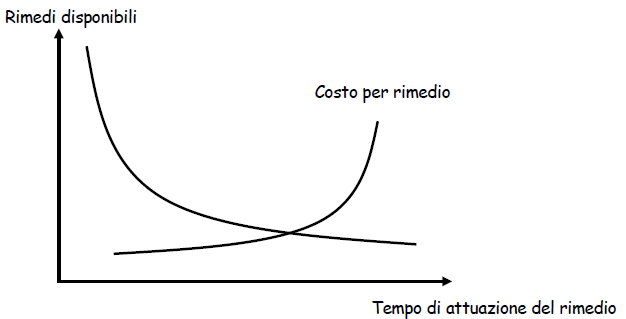
\includegraphics[width=0.7\linewidth]{costo_rimedio.png}
 \centering
 \caption{Rappresentazione del costo per rimedio in funzione del tempo di attuazione}
 \label{fig:costo_rimedio}
\end{figure}
%\newpage
Se il sistema è complesso si può dividere la scheda in più sezioni e analizzare le singole parti,
semplificando le analisi.

Gli ``attori'' che partecipano al fenomeno della compatibilità elettromagnetica sono sicuramente
almeno due: la \textbf{sorgente} e la \textbf{vittima}, tra i due è interposto il canale di accoppiamento.
Il disturbo può colpire la vittima mediante varie \textit{porte} come le porte di comunicazione,
di alimentazione o la porta ``involucro''.

I \textit{canali di accoppiamento} sono le vie utilizzate dai disturbi o dai segnali utili per propagarsi tra i 
dispositivi, il cavo di alimentazione può trasmettere disturbi al dispositivo provenienti dalla rete di alimentazione
ma può essere comunque protetto con un filtro, il discorso si complica per i canali di accoppiamento non previsti,
ovvero canali che non dovrebbero trasmettere alcuna informazione o energia utile per l'apparecchio.

\begin{figure}[h]
 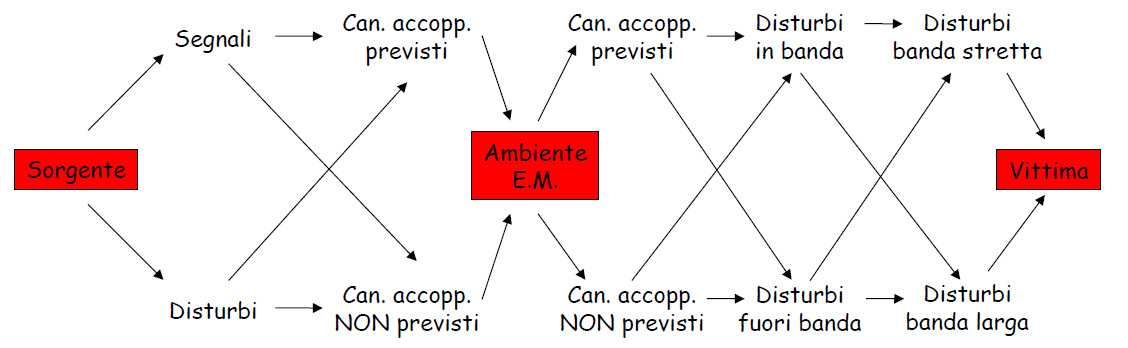
\includegraphics[width=0.7\linewidth]{catena_disturbi.png}
 \centering
 \caption{Rappresentazione della catena dei canali di accoppiamento dei disturbi}
 \label{fig:catena_disturbi}
\end{figure}

I disturbi che si propagano nella vittima possono rientrare o meno nella sua \textbf{banda} di funzionamento
ossia l'intervallo di frequenze alle quali è previsto il funzionamento del dispositivo, un disturbo si dice
a \textit{banda stretta} se rientra nella banda di funzionamento del dispositivo, si dice a \textit{banda larga}
se la sua ampiezza supera la banda di funzionamento del dispositivo.
Un disturbo a banda stretta (\textit{NarrowBand}) probabilmente potrà accoppiarsi con il dispositivo mediante
canali di accoppiamento previsti e risultare udibile per l'utente (ad esempio nel caso di un disturbo radiato che colpisce
un ricevitore FM).
Un disturbo a banda larga (\textit{BroadBand}) non rientra nelle caratteristiche di funzionamento del dispositivo
e potrà utilizzare con buona probabilità anche canali non previsti.
Un segnale composto da una singola componente in frequenza è un segnale a banda stretta per antonomasia.
\begin{figure}[h]
 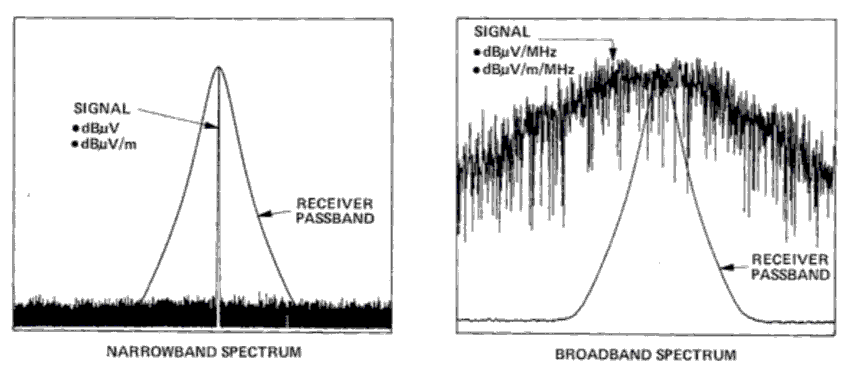
\includegraphics[width=0.7\linewidth]{narrow-broadband.png}
 \centering
 \caption{Confronto tra segnali a banda stretta e larga rispetto al filtro di un ricevitore}
 \label{fig:narrow-broadband}
\end{figure}








\section{Le unità di misura}
Le grandezze di interesse nel campo della Compatiiblità Elettromagnetica sono prevalentemente
campi elettrici [V/m] e magnetici [A/m], e tensioni [V] e correnti [I].
Queste grandezze variano con valori compresi tra $10^{-6}$ e $10^{2}$. C'è una dinamica di ben 8 ordini di grandezza.

Per gestire range così elevati, viene spesso utilizzata la rappresentazione su scale \textit{logaritmiche}.
Proprietà utili del logaritmo sono le seguenti:
\begin{itemize}
 \item [] Somma e differenza: $Y = aX/b \Rightarrow \log(Y) = \log(a) + \log(X) - \log(b) $
 \item [] Prodotto per uno scalare: $Y = 10^x \Rightarrow \log(Y) = x\log(10) $
\end{itemize}

È stato poi introdotto il ``decibel'' definito come:
$$\si{dB}(x) = 10\log_{10}x $$
Spesso si utilizza il deciBel per esprimere un guadagno o un'attenuazione di un amplificatore o un'antenna,
questa unità rappresenta quindi il rapporto tra due grandezze, in genere uscita e ingresso.
Se si indica un rapporto fra potenze continua a valere la precedente definizione ma per comodità
se la resistenza di ingresso dell'amplificatore e quella in uscita hanno lo stesso valore, si può ricavare
la seguente forma del deciBel più comoda e valida solo per le tensioni:

$$G_{P,\si{dB}} = 10\log_{10}\left(\frac{P_{out}}{P_{in}} \right) = 
10\log_{10}\left( \frac{V_{out}^2}{R_{out}}\frac{R_{in}}{V_{in}^2} \right) \stackrel{R_{in} = R_{out}}{=}
20\log_{10}\left(\frac{V_{out}}{V_{in}}\right) = G_{V,\si{dB}} $$

L'ampiezza della dinamica, utilizzando il deciBel diventa:
$$10^8 \Rightarrow 20\log_{10}10^8 = 160$$
in questo modo è molto più semplice rappresentare tali valori su una scala o un grafico.
Storicamente l'utilizzo del deciBel è nato dalla necessità dei costruttori di dispositivi audio di indicare
i livelli di volume sonoro e disturbo dato che anche l'orecchio umano percepisce i suoni con una funzione
logaritmica, tendendo ad attenuare i volumi elevati.

Altre forme del deciBel utilizzate sono quelle che fanno riferimento ad un valore fisso,
ad esempio il $\si{dB}\mu V = 20\log_{10}\frac{V}{1 \mu V}$ si indica quindi in deciBel, quanto la tensione
misurata è più grande (o più piccola) rispetto al \textit{microVolt}.

Per le potenze è spesso utile il $\si{dB}mW $ abbreviato $\si{dB}m = 10\log_{10}\frac{W}{1 mW}$.

\paragraph{Esempio potenza in antenna}
Potenza fornita ad un'antenna in funzione del campo elettrico emesso
$$P_T = G_T \frac{\lambda^2}{4\pi}\frac{E_T^2}{Z_0}$$
Supponiamo una variazione di $6 \si{dB}$ della potenza in antenna, a quanto corrisponde numericamente?
$$6\si{dB} = 10\log_{10}\left(\frac{P_2}{P_1} \right) = 10\log_{10}\left(\frac{E_2}{E_1}\right)^2 =
20\log_{10}\left(\frac{E_2}{E_1}\right) \Rightarrow$$

$$\Rightarrow
\begin{cases}
P_2 = 10^{\frac{6}{10}}\cdot P_1 \approx 4\cdot P_1 \\
E_2 = 10^{\frac{6}{20}}\cdot E_1 \approx 2\cdot E_1
\end{cases}
$$

Il guadagno è sempre adimensionale perchè esprime il rapporto tra grandezze identiche.

\paragraph{Propagazione in linea di trasmissione}



\section{Sorgenti e ricevitori di segnale}

\begin{figure}[h]
\centering
\begin{subfigure}[t]{0.4\textwidth}
\begin{circuitikz}
\draw
(0,0) to [sinusoidal voltage source, l=$V_s$] (0,2)
        to [resistor,-o,l=\mbox{$R_s$}, a=\SI{50}{\ohm}] (3.5,2)
(0,0) to [short , -o] (3.5,0)
;
\draw [dashed] (-0.5,-0.3) rectangle (3,2.25)
;
\end{circuitikz}
\caption{Generatore di disturbi}
\end{subfigure}
\ 
\begin{subfigure}[t]{0.4\textwidth}
\begin{circuitikz}
\draw
(0,0) to [open, o-o] (0,2)
        to [short] (3.5,2)
        to [resistor , l=\parbox{2cm}{$R_{in}\\ \SI{50}{\ohm}$}] (3.5,0)
        to [short] (0,0)
(2.5,0)   to [capacitor, l=\parbox{1.1cm}{\flushright $C_{in}$\\ \SI{0.47}{\pico\farad}}] (2.5,2)
;
\draw [dashed] (0.7,-0.3) rectangle (4.6,2.25)
;
\end{circuitikz}
\caption{Ricevitore di segnale}
\end{subfigure}
\end{figure}



Un filtro con risposta in frequenza molto stretta, richiede una risposta nel tempo
molto ampia, ossia richiede molto tempo per andare a regime.

Fissata una RBW del filtro intermedio a \SI{3}{\decibel}, si avrà in uscita
un segnale composto dalla $f_{\text{if}}$ e da alcune componenti laterali, ossia
un segnale modulato in ampiezza la cui portante è proprio la $f_{\text{if}}$.
L'unione dei picchi nel tempo del segnale viene chiamato \textbf{inviluppo} del segnale,
è in realtà la parte ``interessante'' del segnale che viene infatti inviato
al \textit{rivelatore di inviluppo} che trasforma il segnale modulato nel suo inviluppo.

\begin{figure}[h] %ricevitore di inviluppo
\centering
 \begin{circuitikz}[american voltages]
 \draw
 (0,2) to [full diode,o-] (2,2)
       to [resistor] (2,0)
 (0,0) to [short, o-] (2,0)
 ;
 \draw
 (-0.5,2) to [open, v=$V_{\text{in}}$] (-0.5,0)
 (2.6,2) to [open, v^>=$V_{\text{out}}$] (2.6,0)
 ;
 \end{circuitikz}
 \caption{Rivelatore di inviluppo}
\end{figure}

Quando si ricostruisce il contenuto spettrale del segnale, viene riportato il
valore efficace dell'ampiezza del segnale ad ogni singola frequenza di interesse,
in realtà il valore visualizzato è la somma dei contributi dati dalla componente
in quella frequenza e dalle frequenze \textit{laterali} che rientrano nella 
\textit{Resolution BandWidth}.

Il primo parametro importante da determinare nell'analisi di un segnale
di disturbo è la sua ampiezza massima nel tempo, ossia il suo valore di \textbf{picco}.
L'inviluppo di un segnale infatti può essere variabile nel tempo.

Per questo motivo
il segnale ottenuto con il rilevatore di inviluppo viene inviato ad un filtro passa-basso
comunemente chiamato \textit{Video Pass Bandwidth}, viene quindi eseguita
la media dell'inviluppo. L'ampiezza di banda del filtro passa basso determina
il tempo necessario ad ottenere il valore di media.

Due segnali con lo stesso valore di picco possono però avere inviluppi differenti
in base alla frequenza con la quale il disturbo colpisce il rilevatore.

\begin{figure}[h] %2 circuiti con stesso picco ma periodicità differenti
 \centering
 \begin{subfigure}[t]{0.3\textwidth}
  \begin{circuitikz}
   \draw (0,0)[->] -- (4,0) node[right]{$t$};
   \draw (0,0)[->] -- (0,2) node[left]{$A(t)$};
   \draw (0.1,0) \foreach \k in {0,...,8} { let \n1={1.8*(-2*mod(\k,2) + 1)}
   in -- ++(0,\n1) -- ++(0.4,0)};
   \draw (3.7,0) -- (3.7,1.8);
  \end{circuitikz}
  \caption{}
  \label{fig:segnale_alta_periodicità}
 \end{subfigure}
 \quad \quad \quad
 \begin{subfigure}[t]{0.3\textwidth}
  \begin{circuitikz}
   \draw (0,0)[->] -- (4,0) node[right]{$t$};
   \draw (0,0)[->] -- (0,2) node[left]{$A(t)$};
   \draw (0.1,0) \foreach \k in {0,1} { let \n1={1.8*(-2*mod(\k,2) + 1)}
   in -- ++(0,\n1) -- ++(0.4,0)};
   
   \draw (1.7,0) \foreach \k in {0,1} { let \n1={1.8*(-2*mod(\k,2) + 1)}
   in -- ++(0,\n1) -- ++(0.4,0)};
  
  \draw (3.3,0) \foreach \k in {0} { let \n1={1.8*(-2*mod(\k,2) + 1)}
   in -- ++(0,\n1) -- ++(0.4,0)};
  \draw (3.7,0) -- (3.7,1.8);
  \end{circuitikz}
  \caption{}
  \label{fig:segnale_bassa_periodicità}
 \end{subfigure}
 \caption{}
\end{figure}

Come si vede il segnale in figura \ref{fig:segnale_alta_periodicità} ha un peso 
maggiore rispetto a quello in figura \ref{fig:segnale_bassa_periodicità} dato
che colpisce il ricevitore un numero maggiore di volte nella stessa unità
di tempo.
Il rivelatore di picco non è quindi in grado di discernere la differenza tra i due
segnali.

Si definisce quindi il valore di \textbf{Quasi Picco} quello ottenuto con l'aggiunta
di un condensatore in parallelo alla resistenza del rilevatore di picco, se ne riporta
al display del misuratore il suo valore medio.

La visualizzazione dei valori sul display viene pilotato mediante un generatore
di rampa che permette la traslazione della frequenza dell'oscillatore locale
e la traslazione sull'asse delle frequenze dello schermo.


\section{Analizzatore di spettro o ricevitore di interferenza?}
Si elencano le principali differenze tra i due strumenti principali
utilizzati nella misura dei disturbi: l'\textbf{analizzatore di spettro} e il \textbf{ricevitore di interferenze}.

\begin{center}%tabella emi receiver vs spectrum analyzer
\begin{tabular}{|>{\centering}m{4cm}|>{\centering}m{4cm}|m{4cm}<{\centering}|}
 \rowcolor{blue}
 \hline
  \color{white}\textbf{Parametro}&\color{white}\textbf{Spectrum analyzer} &\color{white} \textbf{EMI receiver} \\
  \hline
  Principio di funzionamento & Spazzolata (sweeped) & Frequenze discrete (\textit{tuned}) \\
  \hline 
  RBW [\si{\kilo\hertz}] &1, 3, 10, 30, 100, ... & 0.2, 9, 120 \\
  \hline
  Banda & \SI{3}{\decibel} & \SI{6}{\decibel} \\
  \hline
  Rivelatore & Pk & (Pk), QP, AVG\\
  \hline
  Selettività e preamplificazione & $-$ & $+$ \\
  \hline
  Accuracy (A \& f) & $-$ & $+$ \\
  \hline
  Resistenza all'overload & $\sim$ & $+$ \\
  \hline
  Costo & $-$ & $++$ \\
  \hline
  Applicazioni & Pre compliance & Full compliance \\
  \hline
\end{tabular}
\end{center}

La definizione di \textit{banda} per i due strumenti è differente,
nell'\textit{analizzatore di spettro} la \textit{resolution bandwidth} 
è l'ampiezza dell'intervallo i cui valori vengono attenuati ad una differenza di massimo 
\SI{3}{\decibel} dal valore
del segnale alla frequenza centrale del filtro.
Questo valore nel \textit{ricevitore di interferenze} è pari a \SI{6}{\decibel}.

L'analizzatore di spettro esegue un'analisi rapida, riportando solo
il valore di picco dell'inviluppo. L'EMI receiver
dispone anche dei rilevatori di QuasiPicco ed Average, il rivelatore
di Picco non è necessario al fine delle verifiche in campo civile.

La \textbf{selettività} indica quanto rapidamente un filtro tende
a 0, anche se 2 filtri hanno la stessa RBW, i valori al di fuori della banda
possono attenuarsi con pendenze diverse.
La \textbf{preamplificazione} è necessaria alla corretta analisi di segnali
di disturbo ad una determinata frequenza che, se di ampiezza bassa, possono
essere confusi con il rumore di fondo dal rilevatore.

L'\textbf{accuracy} è maggiore nell'EMI receiver.
La resistenza all'\textbf{overload} è la resistenza al sovraccarico
degli stadi di ingresso, l'analizzatore di spettro non prevede
segnali in ingresso distruttivi dato che viene prevalentemente usato in 
ambienti controllati o comunque con segnali noti, cosa non vera
per l'EMI receiver, con il quale si misurano disturbi di cui non 
conosciamo preventivamente l'entità.

Il costo di un EMI receiver è molto più alto di quello
di un analizzatore di spettro.
L'analizzatore di spettro permette l'esecuzione
di prove pre-compliance, utili ad avere un'idea dei
possibili problemi di compatibilità, per aver la conformità
alla direttiva è invece necessario il ricevitore di interferenze.

Come si è visto la differenza principale tra i due strumenti consta nella 
selettività e nella preamplificazione, nell'EMI receiver
infatti, in aggiunta a quanto presente anche nell'analizzatore di spettro
è necessario aggiungere un \underline{attenuatore} contro gli 
overload e un \underline{filtro passabanda} necessario a limitare la potenza
in ingresso al mixer per ridurre al minimo gli errori dovuti alla non linearità.
Deve essere inoltre presente un \underline{preamplificatore} necessario ad
innalzare il valore di segnali particolarmente bassi.

Il \underline{preselettore} deve lavorare su ampie gamme di frequenze e non
è richiesto che sia molto stretto, deve solo limitare l'energia
in ingresso al mixer, non svolge alcuna funzione di misura.

\paragraph{Rivelatore di Picco e QuasiPicco}
Il seguente circuito rappresenta uno schema del rivelatore di Picco o di QuasiPicco,
la differenza tra i due rivelatori si ottiene modificando opportunamente la resistenza
di scarica $R_d$.

\begin{figure}[h] %rivelatore di picco
\centering
 \begin{circuitikz}[american voltages]
 \draw
 (0,2) to [full diode,o-,v=$V_d$] (2,2)
       to [resistor,l=$R_c$] (4,2)
       to [capacitor,l=$C$] (4,0)
 (4,2) to [short,-o] (7,2)   
 (6,2) to [resistor,l=$R_d$] (6,0)
 (0,0) to [short, o-o] (7,0)
 ;
 \draw
 (-0.5,2) to [open, v=$V_{\text{in}}$] (-0.5,0)
 (7.6,2) to [open, v^>=$V_{\text{out}}$] (7.6,0)
 ;
 \end{circuitikz}
 \caption{Rivelatore di picco}
\end{figure}

Il rivelatore di Picco ha una resistenza di scarica $R_d$ molto elevata,
il rivelatore di quasipicco invece ha una resistenza di valore confrontabile
con quello della resistenza di carica $R_c$.

Bisogna tenere in considerazione il tempo di misura affinché i valori
misurati, rispettivamente di picco o quasipicco, siano
effettivamente i massimi valori assunti dal segnale e bisogna assicurarsi che
i rivelatori siano andati a regime, i tempi di misura per ogni frequenza possono
essere anche dell'ordine delle centinaia di millisecondi.


\paragraph{Rivelatore di media}
Il seguente rivelatore si ottiene aggiungendo al rivelatore di QuasiPicco 
un filtro passa-basso.

\begin{figure}[h] %rivelatore di media
\centering
 \begin{circuitikz}[american voltages]
 \draw
 (0,2) to [full diode,o-,v=$V_d$] (2,2)
       to [resistor,l=$R_c$] (4,2)
       to [capacitor,l=$C$] (4,0)
 (4,2) to [short] (6,2)   
 (6,2) to [resistor,l=$R_d$] (6,0)
 (6,2) to [resistor] (9,2)
       to [short, -o] (10,2)
 (9,0) to [variable capacitor] (9,2)      
 (0,0) to [short, o-o] (10,0)
 ;
 \draw
 (-0.5,2) to [open, v=$V_{\text{in}}$] (-0.5,0)
 (10.6,2) to [open, v^>=$V_{\text{out}}$] (10.6,0)
 ;
 \draw [dashed] (6.8,-0.3) rectangle (9.6,2.3);
 \end{circuitikz}
 \caption{Rivelatore di media}
\end{figure}

Al variare della capacità variabile presente nel
filtro passa-basso si seleziona la frequenza da analizzare.

%\section{Caratteristiche dei rivelatori}
Le caratteristiche dei rivelatori di QuasiPicco e Media sono riportate nella norma
CISPR 16-1 (EN55016), le informazioni riguardo il rivelatore di Picco sono meno
dettagliate.
Se i valori misurati dal rilevatore di picco e QuasiPicco
coincidono, si può affermare che l'inviluppo del segnale è costante, ossia il
segnale è a onda continua, anche il rilevatore di media indicherà lo stesso valore.

\begin{center} %tabella parametri cispr 16
 \begin{tabular}{|>{\centering}m{3cm}|>{\centering}m{3cm}|>{\centering}m{3cm}|m{3cm}<{\centering}|}
  \hline
  \multicolumn{4}{|c|}{Banda CISPR} \\
  \hline
  &Banda A $9\sim150$\si{\kilo\hertz} & Banda B $0.15\sim30$\si{\mega\hertz} & Banda C $+$ D $30\sim300\sim1000$ \si{\mega\hertz} \\ \hline
  Ampiezza di banda \SI{-6}{\decibel} [\si{\kilo\hertz}] & 0.20 & 9 & 120 \\ \hline
  Costante di \underline{carica} [\si{\milli\second}]   & 45   & 1 & 1 \\ \hline
  Costante di \underline{scarica} [\si{\milli\second}]  & 500  & 160 & 550 \\ \hline
  \rowcolor{yellow}
  Costante meccanica [\si{\milli\second}] & 160 & 160 & 100 \\ \hline
  Fattore di sovraccarico dei circuiti che precedono il rilevatore [\si{\decibel}] & 24  & 30  & 43.5 \\ \hline
  Fattore di sovraccarico tra l'amplificatore a valle e lo strumento indicatore [\si{\decibel}] &  6 &  12 & 6 \\ \hline
 \end{tabular}
\end{center}

Al di sopra della frequenza di \SI{30}{\mega\hertz} si considerano i disturbi
come radiati.

La costante meccanica è ciò che trasforma un segnale variabile
nel tempo in un segnale costante, ossia rappresenta la costante di tempo
di uno smorzatore meccanico equivalente. La somma di tutti e 3 i tempi 
permette di calcolare la costante di tempo dell'intero rilevatore 
affinché la misura sia corretta.

\paragraph{Filtro a frequenza intermedia}
La figura \ref{fig:filtro_IF} riporta la risposta del filtro a frequenza intermedia con ampiezza
di banda pari a \SI{120}{\kilo\hertz} centrato su una frequenza generica.
\begin{figure}[h]
\centering
 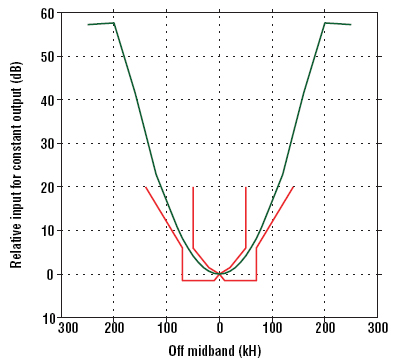
\includegraphics[width=0.6\linewidth]{IF_response}
 \caption{Risposta del filtro IF con ampiezza \SI{120}{\kilo\hertz} (banda \SI{30}{\mega\hertz} $\sim$ \SI{1}{\giga\hertz})}
 \label{fig:filtro_IF}
\end{figure}

L'asse verticale riporta \textit{l'ingresso relativo per un output costante}.
La maschera rossa è quella imposta dalla norma, la curva verde è solo
una possibile risposta del filtro, si può notare come la maschera
\textit{``stringa''} la curva alla frequenza di $\pm$ \SI{60}{\kilo\hertz}
per definire in maniera accurata la banda di \SI{120}{\kilo\hertz} a \SI{-6}{\decibel}.

Viene riportata la maschera fino a \SI{20}{\decibel} per verificare anche la selettività
del filtro, come si nota c'è un ampio margine lasciato al produttore del filtro.
Per permettere la realizzazione di filtri più selettivi, è consentita
una sovraelongazione fino a \SI{1.5}{\decibel} nell'intorno della frequenza centrale.

Il \textbf{rilevatore di media}, mediante il filtro passa-basso permette la rilevazione di componenti ad onda
continua in segnali a banda larga, ossia segnali sinusoidali puri.



\section{Calibrazione dei rivelatori}
I rivelatori di quasi picco e media devono essere necessariamente calibrati
secondo i valori e le metodologie fornite dalla norma.
La prima metodologia di calibrazione analizzata viene chiamata \textbf{assoluta} (in ampiezza), 
si definisce l'area \textit{IS} dell'impulso con la seguente:
$$ %forula area IS dell'impulso
IS = \int_{-\infty}^{+\infty} v(t) dt
$$

Riferendosi alla tabella sottostante, la calibrazione del rivelatore di \textbf{quasi-picco}
viene effettuata mediante l'analisi della risposta agli impulsi con area
\textit{IS} pari ad \textit{a)}, spettro uniforme almeno fino a \textit{b)}, e
frequenza di ripetizione pari a \textit{c)}, deve essere la stessa (entro \SI{1.5}{\decibel}) di un
segnale sinusoidale non modulato di pari frequenza, avente un'ampiezza
di valore efficace pari a \SI{2}{\milli\volt} ossia \SI{66}{\decibel\micro\volt}.

\begin{center} %tabella parametri calibrazione assoluta quasipico
 \begin{tabular}{|>{\centering}p{4cm}|>{\centering}p{2.8cm}|>{\centering}p{2.8cm}|p{2.8cm}<{\centering}|}
  \hline
    \textbf{Frequency range} & \textbf{a)} \si{\micro\volt\second} & \textbf{b)} \si{\mega\hertz} & \textbf{c)} \si{\hertz} \\ \hline
    \SI{9}{\kilo\hertz} to \SI{150}{\kilo\hertz}     & 13.5  & 0.15 & 25  \\ \hline
    \SI{150}{\kilo\hertz} to \SI{30}{\mega\hertz}    & 0.316 & 30   & 100 \\ \hline
    \SI{30}{\mega\hertz} to \SI{300}{\mega\hertz}    & 0.044 & 300  & 100 \\ \hline
    \SI{300}{\mega\hertz} to \SI{1000}{\mega\hertz}  & 0.044 & 1000 & 100 \\ \hline
 \end{tabular}
\end{center}

Si analizza ora la calibrazione \textbf{relativa} (in frequenza).
Seguendo la curva in figura \ref{fig:calibrazione_relativa} si valuta 
la variazione di \textit{ampiezza} da dare al segale al variare
della frequenza di ripetizione per ottenere sempre la stessa
indicazione di quasi-picco dallo strumento.

\begin{figure}[h] %figura calibrazione relativa quasi-picco
 \centering
 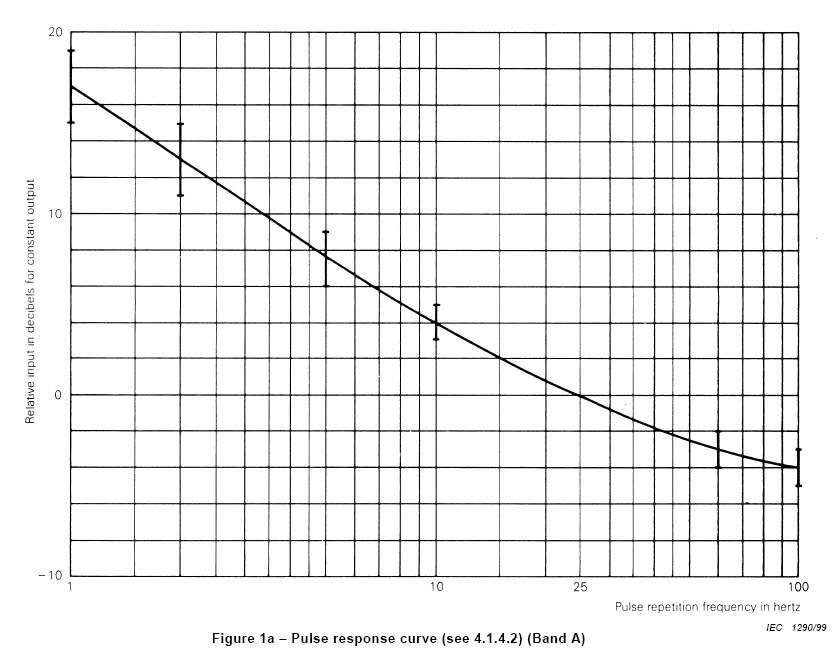
\includegraphics[width=0.7\textwidth]{calibrazione_relativa}
 \caption{Valore del segnale da fornire al variare della frequenza di ripetizione}
 \label{fig:calibrazione_relativa}
\end{figure}

\paragraph{Rilevatore di picco}
Per questo rilevatore viene specificata l'ampiezza di banda a \SI{-6}{\decibel} con
una banda aggiuntiva (Banda E) per segnali superiori a \SI{1}{\giga\hertz}, in questo
caso la banda dell'impulso di riferimento viene calcolata mediante la seguente
$$ %formula B_{imp}
 B_{\text{imp}} = A(t)_{\text{max}} / 2G_0 \cdot IS
$$

I valori per le altre bande sono definiti in tabella:

\begin{center} %tabella parametri banda picco
 \begin{tabular}{|>{\centering}m{5cm}|>{\centering}m{3.2cm}|m{3.2cm}<{\centering}|}
  \hline
    \textbf{Frequency range} & \textbf{Bandwidth $B_6$} & \textbf{Reference BW}  \\ \hline
    \SI{9}{\kilo\hertz}   to \SI{150}{\kilo\hertz}  (A)   & \SI{100}{\hertz}      to \SI{300}{\hertz}      & \SI{200}{\hertz}      \\ \hline
    \SI{150}{\kilo\hertz} to \SI{30}{\mega\hertz}   (B)   & \SI{8}{\kilo\hertz}   to \SI{10}{\kilo\hertz}  & \SI{9}{\kilo\hertz}   \\ \hline
    \SI{30}{\mega\hertz}  to \SI{1000}{\mega\hertz} (C+D) & \SI{100}{\kilo\hertz} to \SI{500}{\kilo\hertz} & \SI{120}{\kilo\hertz} \\ \hline
    \SI{3}{\giga\hertz}   to \SI{18}{\giga\hertz}   (E)   & \SI{300}{\kilo\hertz} to \SI{2}{\mega\hertz}   & \SI{1}{\mega\hertz}   \\ \hline
 \end{tabular}
\end{center}

A differenza delle caratteristiche specifiche del rilevatore di quasi-picco,
per quanto riguarda le \textbf{costanti} di carica e di scarica, viene
definito dalla CISPR il \textit{rapporto minimo fra la costante di scarica e carica
che consente di raggiungere un'indicazione entro il 10\% del valore di picco con un segnale
con frequenza di ripetizione di \SI{1}{\hertz}}
\begin{itemize} % elenco rapporti tra le costanti di carica e scarica picco
 \item [a)] $1.89\cdot10^4$ in banda A   (\SI{9}{\kilo\hertz}   $\sim$ \SI{150}{\kilo\hertz})
 \item [b)] $1.25\cdot10^6$ in banda B   (\SI{150}{\kilo\hertz} $\sim$ \SI{30}{\mega\hertz})
 \item [c)] $1.67\cdot10^7$ in banda C+D (\SI{30}{\mega\hertz}  $\sim$ \SI{1000}{\mega\hertz})
 \item [d)] $1.34\cdot10^8$ in banda D   (\SI{1}{\giga\hertz}   $\sim$ \SI{18}{\giga\hertz})
\end{itemize}

Si definisce inoltre la risposta agli impulsi di area 
pari a $1.4/B_{\text{imp}}$ \si{\milli\volt\second} che deve essere pari a quella
fornita per un segnale sinusoidale di valore efficace \SI{2}{\milli\volt} (\SI{66}{\decibel\micro\volt})

\begin{table}[h] %tabella risposta agli impulsi Picco table generated on tablesgenerator.com
\centering
%\resizebox{\textwidth}{!}{%
\begin{tabular}{|c|c|c|c|c|}
\hline
\multirow{3}{*}{Frequency} & \multirow{3}{*}{\makecell{ IS \\ \si{\milli\volt\second}}} & \multirow{3}{*}{\makecell{$B_{\text{imp}}$\\ \si{\hertz}}} &
\multicolumn{2}{c|}{\multirow{2}{*}{\makecell{Ratio peak/quasi-peak (\si{\decibel})\\ for pulse repetition rate}}} \\
                           &       &        & \multicolumn{2}{c|}{}   \\ \cline{4-5} 
                           &       &        & 25 \si{\hertz}          & 100 \si{\hertz}     \\ \hline
Band A                     & 6.67  & $0.21\cdot10^3$   & 6.1          & $-$                 \\ \hline
Band B                     & $0.148\cdot10^{-3}$       & $9.45\cdot10^3$   & $-$            & 6.6       \\ \hline
Band C + D                 & $0.011\cdot10^{-3}$       & $126.0\cdot10^3$  & $-$            & 12.0      \\ \hline
\end{tabular}%
%}
\end{table}

Come si vede in tabella, il rilevatore di picco viene confrontato con un rilevatore
di quasi-picco già conforme alle norme CISPR.

Anche per quanto riguarda il rilevatore di \textbf{media} viene utilizzata una tabella
con i parametri dell'ampiezza di banda del rivelatore.

\begin{center} %tabella parametri banda media
 \begin{tabular}{|>{\centering}m{5cm}|>{\centering}m{3.2cm}|m{3.2cm}<{\centering}|}
  \hline
    \textbf{Frequency range} & \textbf{Bandwidth $B_6$} & \textbf{Reference BW}  \\ \hline
    \SI{9}{\kilo\hertz}   to \SI{150}{\kilo\hertz}  (A)   & \SI{100}{\hertz}      to \SI{300}{\hertz}      & \SI{200}{\hertz}      \\ \hline
    \SI{150}{\kilo\hertz} to \SI{30}{\mega\hertz}   (B)   & \SI{8}{\kilo\hertz}   to \SI{10}{\kilo\hertz}  & \SI{9}{\kilo\hertz}   \\ \hline
    \SI{30}{\mega\hertz}  to \SI{1000}{\mega\hertz} (C+D) & \SI{100}{\kilo\hertz} to \SI{500}{\kilo\hertz} & \SI{120}{\kilo\hertz} \\ \hline
    \SI{3}{\giga\hertz}   to \SI{18}{\giga\hertz}   (E)   & \SI{300}{\kilo\hertz} to \SI{2}{\mega\hertz}   & \SI{1}{\mega\hertz}   \\ \hline
 \end{tabular}
\end{center}

Per quanto riguarda la calibrazione in ampiezza invece, per impulsi di area pari a 
1.4/n \si{\milli\volt\second} con frequenza di ripetizione pari a n \si{\hertz},
la risposta deve essere pari a quella fornita per un segnale sinusoidale di valore efficace
pari a 2 \si{\milli\volt} (\SI{66}{\decibel\micro\volt}).

\begin{table}[h] %tabella risposta agli impulsi Media (sempre su tablesgenerator.com) Non impazzire con il codice di latex!!!
\centering
\begin{tabular}{|c|c|c|c|c|c|}
\hline
\multirow{3}{*}{Frequency} & \multicolumn{5}{c|}{\multirow{2}{*}{Ratio quasi-peak/average (\si{\decibel}) for pulse repetition rate}} \\
                           & \multicolumn{5}{c|}{}                                                                                 \\ \cline{2-6} 
                           & \SI{25}{\hertz}    & \SI{100}{\hertz}   & \SI{500}{\hertz}   & \SI{1000}{\hertz}  & \SI{5000}{\hertz} \\ \hline
Band A                     & 12.4               &                    &                    &                    &                   \\ \hline
Band B                     &                    & (32.9)             & 22.9               & (17.4)             &                   \\ \hline
Band C + D                 &                    &                    &                    & (38.1)             & 26.3              \\ \hline
\end{tabular}
\end{table}

Le caratteristiche comuni dell'ampiezza di banda permettono ai costruttori degli strumenti
di misura di realizzare un unico filtro a frequenza intermedia con le stesse
caratteristiche per tutte e tre le tipologie di misura.




\section{Segnali a banda stretta e banda larga}
Si definisce segnale a \textit{banda stretta} per antonomasia, un segnale sinusoidale
con una sola componente spettrale ma in generale
si definisce un segnale a banda stretta se il suo contenuto spettrale
sia interamente contenuto nella banda del filtro a frequenza intermedia.
Se il suo contenuto spettrale è al di fuori dell'ampiezza del filtro,
viene definito segnale a \textit{banda larga}.

Sia dato un segnale ad onda quadra così definito:
$$
x(t) = \sum_{k = -\infty}^{+\infty} A\cdot p\left(\frac{t-kT}{\tau}\right)
$$

La sua trasformata di Fourier è la seguente:
$$
x(f) = 2 \frac{A\tau}{T} \sum_{k=-\infty}^{+\infty} \text{sinc} \left(\pi \frac{k\tau}{T}\cdot  \delta\left(f-\frac{k}{T}\right)  \right)
$$

ossia un treno di impulsi con una distanza pari a $1/T$ e modulati
da una \textit{sinc} con impulsi che si azzerano in multipli di $1/\tau$.

Supponiamo di analizzare un segnale composto da impulsi ad onda quadra,
analizziamo l'intero spettro in un certo tempo $t$ definito come \textit{sweep time}
ossia il tempo necessario a passare dalla frequenza minima a quella massima,
il segnale però è presente soltanto durante la presenza dell'impulso.

\begin{figure}[h] %%grafico linee scansione sweep time
    \centering
    \def\svgwidth{0.6\columnwidth}
    \input{img/grafico.pdf_tex}
\end{figure}


Supponiamo di avere uno sweep time multiplo n-esimo
del tempo di ripetizione del segnale, rileveremo con una sola ``sweppata''
soltanto alcune frequenze, le frequenze analizzate durante il periodo di \textit{off}
del segnale, essa non verrà rilevata, l'esito dell'analisi sarà quindi povera di campioni,
la sua ricostruzione non restituirebbe il segnale originale.

Per ovviare a questo problema si può ridurre lo sweep time ed effettuare più scansioni
ripetute, conservando tutti i campioni raccolti si può (dopo un numero significativo di sweeppate)
ricostruire il segnale di partenza. Si può anche supporre che il tempo totale necessario ad effettuare
la misura sia lo stesso.
Si può inoltre affermare che il segnale sia di tipo ``impulsivo'' data l'assenza di campioni in
alcune misurazioni, determinato ciò, vanno determinati $T$ e $\tau$.
$T$ è la distanza tra 2 impulsi, utilizzando il grafico ottenuto con lo sweep lungo,
possiamo ricavare $T$ con la seguente:
$$
    \frac{\text{SWT}}{\text{SPAN}} = \frac{T}{\Delta f} \Rightarrow T = \frac{\text{SWT}\cdot\Delta f}{\text{SPAN}}
$$
%%% 1:00:30
La misura con uno sweep time breve permette di ottenere una rappresentazione
più accurata delle componenti presenti nel segnale.

Per calcolare il parametro $\tau$ invece si può utilizzare uno sweep time
abbastanza lungo da ottenere tutte le frequenze ravvicinate nella stessa analisi, facendo 
in questo modo, si possono determinare i punti a frequenza nulla, l'ampiezza
della ``onda'' è pari a $1/\tau$.

Usando lo sweep-time breve invece si può associare ad un \textbf{max hold},
un componente presente nel detector che conserva i risultati delle ``spazzolate'' precedenti,
utile anche in questo caso al calcolo di $\tau$.



\paragraph{EMI receiver}

Questo dispositivo lavora con frequenze discrete, seleziona
una frequenza ed esegue la misura, poi l'oscillatore locale
avanza di una frequenza pari a $RBW/2$ ovvero mezza Resolution Bandwidth,
il tempo necessario ad eseguire la misura è molto maggiore a causa dei tempi
tipici dei vari rivelatori.

il \textit{Test della resolution bandwidth} permette di determinare
se il segnale è a banda stretta o larga, se il segnale è a banda stretta, il valore
misurato non dipende dall'ampiezza della Resolution Bandwidth (a meno del rumore addizionale),
nel caso di segnale a banda larga invece possiamo determinare un valore della Resolution Bandwidth oltre
il quale l'ampiezza non varia ulteriormente.
Questa procedura non è comunque esaustiva al fine della determinazione delle caratteristiche di 
ampiezza di banda del segnale.
%% inserisci figura 0:31

Un altro metodo è il confronto tra i valori dei rivelatori di picco e media,
il rivelatore di picco è sensibile a tutta la potenza del segnale presente nella
resolution bandwidth, mentre il rivelatore di average è sensibile prevalentemente al peso
del segnale alla frequenza centrale del filtro, se il valore di picco è superiore di \SI{6}{\decibel}
rispetto al valore di media, allora il segnale sarà a banda larga, se questa differenza
è inferiore a \SI{6}{\decibel} allora sarà a banda stretta.

\section{Disturbi radiati e disturbi condotti}
Esistono in Europa due range di frequenze per caratterizzare i disturbi radiati:
\begin{itemize}
 \item [FCC:] \SI{30}{\mega\hertz} ($\lambda = $ \SI{10}{\meter}) $\rightarrow$ \SI{40}{\giga\hertz} ($\lambda = $ \SI{7,5}{\milli\meter})
 \item [CISPR:] \SI{30}{\mega\hertz} ($\lambda = $ \SI{10}{\meter}) $\rightarrow$ \SI{1}{\giga\hertz} ($\lambda =$ \SI{30}{\centi\meter})
\end{itemize}

Entrambi gli enti normativi definiscono 2 categorie di oggetti da sottoporre a prove di compatibilità elettromagnetica,
\begin{itemize}
 \item [Classe A:] destinati all'industria pesante
 \item [Classe B:] destinati all'uso domestico e commerciale o industria leggera
\end{itemize}

\begin{figure}[h]
\begin{center}
\begin{tabular}{|c|c|c|}
  \hline
       & Classe A        & Classe B       \\ \hline
 FCC   & \SI{10}{\meter} & \SI{3}{\meter} \\ \hline
 CISPR & \SI{10}{\meter} &\SI{10}{\meter} \\ \hline
\end{tabular}
\end{center}
\caption{Distanza a cui effettuare le misure}
\end{figure}

Il diverso ambiente in cui questi oggetti devono funzionare rende necessaria la differente
analisi, gli oggetti di industria pesante sono solitamente di dimensioni maggiori,
questo rende necessario effettuare una misura a grande distanza per assicurarsi che 
ci si trovi in condizione di \textit{campo lontano}.

Nel caso in cui questa distanza non possa essere mantenuta, si effettua una misura
a distanza inferiore, ad esempio a \SI{3}{\meter} con valori di soglia superiori.

Sappiamo che il campo elettrico si propaga come:
$$
 \left|E_r \right| \propto \frac{1}{r} 
$$
il livello di campo a \SI{3}{\meter} si può calcolare:

$$
 \frac{E_3}{E_{10}} = \frac{r_{10}}{r_{3}} \Rightarrow 20\log_{10}E_3 - 20\log_{10}E_{10} = 20\log_{10}\left( \frac{10}{3}\right) \simeq \SI{10}{\decibel}
$$
$$
 E_3 \simeq 3\cdot E_{10}
$$

\section{Correnti di modo comune e correnti di modo differenziale}
Le correnti di \textbf{modo comune} si hanno solitamente quando sono presenti masse
a potenziali diverse oppure sono presenti asimmetrie o imperfezioni nelle schede elettroniche.
Le correnti di \textbf{modo differenziale} invece sono solitamente quelle necessarie al
corretto funzionamento di qualsiasi dispositivo elettrico o elettronico.

\begin{figure}[h] %1:15 aggiungi figura
\centering
 \begin{circuitikz}
 \draw
 (0,0) [dashed] -- (4,0)
 ;
 \end{circuitikz}
\end{figure}

Dalla figura si può vedere che il contributo di disturbo dato dalle
correnti di modo comune genera un campo nel punto 2 superiore a quello
generato dalle correnti di modo differenziale supponendo che la corrente nei conduttori sia la stessa.
Anche in caso di corrente di modo comune di intensità più bassa può comunque avere un'entità di disturbo
paragonabile a quello dato dalle correnti di modo differenziale.



Se avessimo una scheda elettronica con un generatore ed un carico,
si avrebbero due conduttori, i quali sarebbero attraversati dalla corrente
differenziale, si può supporre che si sia anche una corrente
di modo comune aggiuntiva, dovuta a causa della non idealità dell'ossido,
che si richiuda verso la massa al di sotto della scheda.

$$
\begin{cases}
I_1 = I_C + I_D \\
I_2 = I_C - I_D
\end{cases}
\Rightarrow \quad
\begin{cases}
I_C = \frac{I_1+I_2}{2} \\
I_D = \frac{I_1-I_2}{2}
\end{cases}
$$

Immaginando di avere 2 fili di corrente a distanza $S/2$ dall'origine,
le due correnti procedono nello stesso verso, verso l'asse $Z$.
Per caratterizzare il campo generato possiamo scomporne le componenti lungo i tre assi
ottenendo in ogni punto dello spazio un campo elettrico $E_\theta(r,\theta,\varphi)$.
A grande distanza si vede che il campo elettrico dipende solo dalla variabile $\theta$
$$
 E_\theta = M \cdot I \cdot \frac{e^{-j\beta_0 r}}{r} F(\theta)
$$

$M$ e $F(\theta)$ sono due grandezze che dipendono dal tipo di dipolo considerato, $\beta_0 = 2\pi/\lambda$.

\paragraph{Dipolo Hertziano} È un dipolo \textit{piccolo elettricamente}
ossia piccolo rispetto alla lunghezza d'onda che lo attraversa, se così
non fosse non si potrebbe affermare che il valore della corrente sia
uniforme lungo la sua lunghezza.

I parametri del dipolo hertziano sono i seguenti:
$$
\begin{cases}
M =  2\pi j \cdot 10^{-7} L f \\
F(\theta) = \sin \theta
\end{cases}
$$

I raggi che collegano i due conduttori con il punto di osservazione si possono supporre paralleli
a causa della grande di stanza del punto di osservazione dal dipolo.
Il campo totale $E_T$ sarà pari, applicando il principio di sovrapposizione degli effetti:
$$
 E_T = E_1 + E_2 = M\cdot F(\theta)\cdot \left[\frac{I_1 e^{-j\beta_0 r_1}}{r_1} +\frac{I_2 e^{-j\beta_0 r_2}}{r_2}  \right]
$$

%%0:33 inserisci immagine fili a grande distanza r1 r e r2 cap 9 libro

$\Delta$ è il cammino addizionale rispetto al conduttore più vicino
che il campo deve percorrere per raggiungere il punto P,
$\gamma$ è l'angolo tra la retta che congiunge P all'origine e l'asse Y, di conseguenza
$\Delta$ sarà 
$$
\Delta = \frac{s}{2}\cos\gamma = \frac{s}{2}\cdot \hat{\imath}_y\cdot \hat{\imath}_r
$$

Un altro modo per esprimere $\Delta$ è quello di proiettare prima il punto sul piano XY, successivamente
proiettare il punto ottenuto $\Delta'$ sull'asse Y.
$$
\cos\gamma = \cos\left(\frac{\pi}{2} - \theta\right) \cdot \sin\varphi = \sin\theta \cdot \sin\varphi
$$

Nel complesso
$$
\begin{cases}
r_1 = r + \Delta = r + \frac{s}{2} \sin\theta \sin\varphi \\
r_2 = r - \Delta = r - \frac{s}{2} \sin\theta \sin\varphi
\end{cases}
$$

$$
E_T = 2 \pi j \cdot 10^{-7} L f \frac{e^{-j \beta_0 r}}{2} \left[I_1 e^{-j \beta_0 \Delta} + I_2 e^{j \beta_0 \Delta} \right]\sin\theta
$$

\paragraph{Calcolo campo con correnti di modo differenziale}
In questo caso $I_1 = I_D$ e $I_2 = -I_D$
\begin{equation*}
 \begin{split}
E_D & = 2 \pi j \cdot 10^{-7} L f \frac{I_D}{2}e^{-j \beta_0 r} \left[e^{-j \beta_0 \Delta} - e^{j \beta_0 \Delta} \right]\sin\theta \\
 & = 2 \pi j \cdot 10^{-7} L f \frac{I_D}{2}e^{-j \beta_0 r} \left[-2j\sin(\beta_0\Delta)\right]\sin\theta \\ %%e il meno???
 & = 4\pi\cdot10^{-7}Lf\frac{I_D}{2}e^{-j\beta_0 r} \sin\left(\beta_0 \frac{s}{2} \sin\theta \sin\varphi \right)\sin\theta
  \end{split}
\end{equation*}

Valutando $\left|E_D\right|$ per cercarne il massimo si ottiene
\begin{equation*}
 \begin{split}
\text{max}&\left|E_D\right| = 4\pi\cdot10^{-7}Lf\frac{I_D}{2}\sin\left(\beta_0 \frac{s}{2} \sin\theta \sin\varphi \right)\sin\theta \\
& \stackrel{\theta = \pi/2}{=} 4\pi\cdot10^{-7}Lf\frac{I_D}{2}\sin\left(\frac{2\pi}{\lambda} \frac{s}{2} \sin\varphi \right) 
  \end{split}
\end{equation*}

Possiamo affermare quindi che il valore massimo del campo si trova sul piano XY, ossia quando
$\theta$ è pari a $\pi/2$.
Analizziamo ora la funzione rispetto a $\varphi$, se $s\ll\lambda$ ossia i due conduttori
si trovano ad una distanza molto inferiore rispetto alla lunghezza d'onda, il seno presente nell'equazione
si confonderà con l'argomento del seno stesso:
$$
\left|E_D\right| \stackrel{s\ll\lambda}{=} \frac{4\pi^2\cdot10^{-7}}{r}f\frac{I_D L}{\lambda}s  
$$
In conclusione
$$
\left|E_D \right|_{\text{max}} \stackrel{\theta,\varphi = \pi/2}{=} \frac{4\pi^2\cdot10^{-7}I_D}{c\cdot r}Lsf^2
$$
Se ci si sposta lungo l'asse X, il campo è pari a 0 perchè i percorsi dei differenti campi sono identici,
ma il loro valore è uguale e opposto.




\paragraph{Calcolo campo con correnti di modo comune}
$I_1 = I_2 = I_C$

\begin{equation*}
\begin{split}
E_C & = 2 \pi j \cdot 10^{-7} L f \frac{I_C}{r}e^{-j \beta_0 r} \left[e^{-j \beta_0 \Delta} + e^{j \beta_0 \Delta} \right]\sin\theta \\
\left|E_C\right| & = 2 \pi \cdot 10^{-7} L f \frac{I_C}{r} \cdot 2 \cos(\beta_0\Delta)\sin\theta = \\
& = 4\pi\cdot10^{-7}Lf \frac{I_C}{r}\cos\left.\left(\frac{2\pi}{\lambda}\frac{s}{2}\sin\theta\sin\varphi\right)\sin\theta\right|_{\theta=\frac{\pi}{2}} =\\
& = 4\pi\cdot10^{-7}Lf\frac{I_C}{r}\cos\left.\left(\frac{2\pi}{\lambda}\frac{s}{2} \sin\varphi\ \right)\ \right|_{\varphi=?} \stackrel{s\ll\lambda}{=} 4\pi\cdot10^{-7}Lf\frac{I_C}{r}
\end{split}
\end{equation*}

Si riportano quindi le due espressioni di campo elettrico in funzione delle correnti:

\begin{equation*}
 \begin{split}
 E_D & = \frac{4\pi^2\cdot10^{-7}}{c}\cdot \frac{I_D}{r} f^2 Ls\ \text{con}\ \begin{split}
 \theta & = \pi/2 \\
 \varphi & = \pi/2
 \end{split}\\
 E_C & = 4\pi\cdot10^{-7}\frac{I_C}{r}fL\qquad\ \ \text{con}\ \begin{split}
  \theta & = \pi/2 \\
 \forall& \ \varphi\in R
 \end{split}
 \end{split}
\end{equation*}

\paragraph{Esercizio}
Siano dati i seguenti valori: (Sol. $I_C = \SI{2.4e-6}{\ampere}\quad I_D = \SI{1.8e-3}{\ampere}$)
\begin{equation*}
 \begin{split}
 f & = \SI{100}{\mega\hertz} \qquad L = \SI{1}{\meter} \\
 d & = \SI{3}{\meter}\quad \ \ s = 50\ \text{mil} = 50\cdot 25,4\cdot10^{-6} \si{\meter}
 \end{split}
\end{equation*}
Trova i valori di corrente $I_C$ e $I_D$ tali che si abbia un campo pari a $E = \SI[per-mode=symbol]{100}{\micro\volt\per\meter}$

\newpage

%%inizia pagina nuova
\paragraph{Contromisure}
Lo scopo dell'analisi di compatibilità elettromagnetica è quello di attuare opportune
contromisure per ridurre l'intensità del campo, alcuni parametri delle equazioni sono costanti,
si può quindi agire sulla corrente necessaria al funzionamento del dispositivo
riducendo al minimo $I_D$ affinché funzioni il dispositivo, le correnti $I_C$ invece sono correnti 
dovute a non idealità che vanno quindi ridotte al minimo, ad esempio gestendo al meglio
filtraggi e bilanciamenti, la presenza di masse a potenziale differente.

Un' ulteriore soluzione è la riduzione della frequenza del segnale, in particolare
per il campo di modo differenziale che dipende dal quadrato della frequenza,
la controindicazione è avere un dispositivo che trasporta meno informazioni.

I fattori geometrici come la distanza tra i conduttori e la loro lunghezza influiscono
anch'essi sulla ampiezza del campo emesso, all'aumentare di tali parametri aumenta il campo emesso,
per le correnti di modo comune conta l'\textit{area} mentre per quelle di modo differenziale la \textit{lunghezza}.

Definiamo $E/I$ come la funzione di trasferimento del sistema corrente-campo, ingresso-uscita:
\begin{equation*}
\begin{split}
\frac{E_D}{I_D} & = K(d)f^2 \\
\frac{E_C}{I_C} & = K'(d)f
\end{split}
\end{equation*}
Rappresentiamo il diagramma di Bode della funzione di trasferimento per il campo differenziale:

%%Inserisci diagramma 0:57

Abbiamo una funzione che sale con una pendenza di \SI{+40}{\decibel/dec} mentre nel caso della funzione
di modo comune avremo una pendenza di \SI{+20}{\decibel/dec}, il segnale in ingresso
è un treno di impulsi con parametri $\tau$ il periodo e $\tau_r$ il tempo di salita.
Il diagramma di Bode del segnale parte con una pendenza di \SI{0}{\decibel/dec} e alla frequenza di $1/\pi\tau$
scende con una pendenza di \SI{-20}{\decibel/dec}, in corrispondenza di $1/\pi\tau_r$ continua
a scendere con pendenza \SI{-40}{\decibel/dec}.

Sommando i vari diagrammi si può ottenere il campo in uscita data la corrente.
%%Inserisci diagrammi risultati
Osservando i grafici si può vedere l'andamento di un pacchetto di frequenze che formano il treno %1:08 
di impulsi trapezoidali si vede che il segnale di modo
differenziale raggiunge il picco dopo una certa frequenza, per ridurre l'emissione si può aumentare
$\tau$ e $\tau_r$ ottenendo complessivamente una pendenza più bassa e un valore assoluto del segnale
inferiore, allo stesso modo anche il segnale di modo comune, non è però conveniente ridurre le frequenze dei funzionamento dei dispositivi.
Una soluzione utile per ridurre i disturbi emessi può essere quella di intrecciare i cavi di alimentazione



\end{document}
